
\chapter{\meteorNAME}\label{cap:chapter_meteor}


\meteorNAME es un \environmentPL ultra-simple para construir \websitesINT modernos. Lo que antes demoraba semanas, incluso con las mejoras herramientas, ahora toma horas con \meteorNAME.
%Meteor is an ultra-simple environment for building modern websites. What once took weeks, even with the best tools, now takes hours with Meteor.

La \webINT fue diseñada originalmente para trabajar de la misma manera que los \mainframesAS funcionaban en los 70s. La aplicación del \serverAS \rendered una \screen y la envía a través de la \networkINT a un \dumbterminal (\refFigura{figure:mainframeServer_dumbterminal}). Si el usuario realizó alguna acción, el \serverAS \rendered una \screen completamente nueva. Este modelo funcionó bien para la \webINT por una década. Esto permitió la existencia de \lampNAME, \rails, \djangoNAME, \phpNAME.
%The web was originally designed to work in the same way that mainframes worked in the 70s. The application server rendered a screen and sent it over the network to a dumb terminal. Whenever the user did anything, that server rerendered a whole new screen. This model served the Web well for over a decade. It gave rise to LAMP, Rails, Django, PHP.

\begin{figure}[h!]
	\centering
	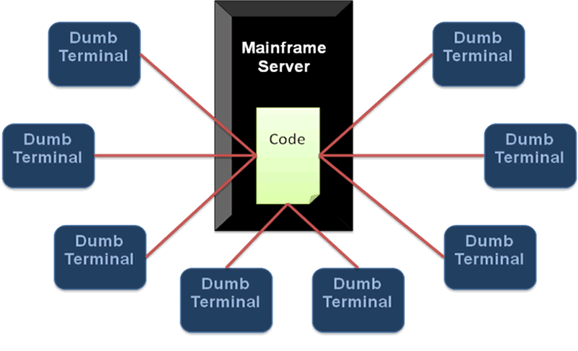
\includegraphics[width=0.6\textwidth]{figuras/mainframeServer_dumbterminal.png}
	\caption{Aquitectura de \mainframeAS con \dumbterminal}
	\label{figure:mainframeServer_dumbterminal}
\end{figure}


Pero los mejores equipos, con los mas grandes presupuestos y mas largos \schedules, ahora construyen aplicaciones en \javaScriptNAME que correr en el \clientAS. Estas aplicaciones tienen interfaces estelares. Estas aplicaciones no \reload \pages, son \reactive: cambios de cualquier \clientAS aparecen inmediatamente en las \screen de todos.
%But the best teams, with the biggest budgets and the longest schedules, now build applications in JavaScript that run on the client. These apps have stellar interfaces. They don't reload pages. They are reactive: changes from any client immediately appear on everyone's screen.

La aplicación fue construida de la manera difícil. \meteorNAME hace esto con la intención de ofrecer simpleza, y muchísima más entretención. Es posible construir una aplicación completa en un fin de semana, o en una \hackathonCPT con la suficiente cafeína. Ya no es necesario los \resourcesCPT del \serverAS, o \deploy \api \apiendpointsAS en la \cloud, o manejar una \dataBaseDB, o desgastarse con una \orm \layer, o intercambiar \backandforth entre \javaScriptNAME y \rubyNAME, o \broadcast datos de invalidación a los \clientsAS.
%They've built them the hard way. Meteor makes it an order of magnitude simpler, and a lot more fun. You can build a complete application in a weekend, or a sufficiently caffeinated hackathon. No longer do you need to provision server resources, or deploy API endpoints in the cloud, or manage a database, or wrangle an ORM layer, or swap back and forth between JavaScript and Ruby, or broadcast data invalidations to clients.

\meteorNAME es un trabajo en desarrollo, pero se espera que muestra la dirección del equipo desarrollador. Ellos están deseosos de recibir \feedback. 
%Meteor is a work in progress, but we hope it shows the direction of our thinking. We'd love to hear your feedback.

\section{Principios de \meteorNAME}
%Principles of Meteor
\begin{itemize}
	\item \textbf{Datos \onthewire}. \meteorNAME no envía \htmlNAME a través de la \networkINT. El \serverAS envía datos y permite al \clientAS \render la información.
%Data on the Wire. Meteor doesn't send HTML over the network. The server sends data and lets the client render it.

	\item \textbf{Un lenguaje}. \meteorNAME permite escribir el código correspondiente al \clientAS y a el \serverAS de la aplicación en \javaScriptNAME.
%One Language. Meteor lets you write both the client and the server parts of your application in JavaScript.
	\item \textbf{\dataBaseDB en todas partes}. Se pueden utilizar los mismos métodos para acceder a la \dataBaseDB desde el \clientAS o el \serverAS.
%Database Everywhere. You can use the same methods to access your database from the client or the server.

	\item \textbf{Compensación de \latency}. En el \clientAS, \meteorNAME \prefetches datos y simula modelos para aparentar que los métodos del \serverAS retornan instantáneamente.
%Latency Compensation. On the client, Meteor prefetches data and simulates models to make it look like server method calls return instantly.

	\item \textbf{\fullstackAS \reactivity}. En \meteorNAME, \realTimeINT es el \default. Todas las \layers, desde la \dataBaseDB hasta el \templateAS, \update por si mismo automáticamente cuando es necesario.
%Full Stack Reactivity. In Meteor, realtime is the default. All layers, from database to template, update themselves automatically when necessary.

	\item \textbf{\embraceecosystem}. \meteorNAME es un \openSourcePC e integra \tools y \frameworksPC \openSourcePC.
%Embrace the Ecosystem. Meteor is open source and integrates with existing open source tools and frameworks.

	\item \textbf{\simplicity igual \productivity}. La mejor manera para de hacer algo que parezca sencillo es tener lo que realmente sea simple. La principal funcionalidad de \meteorNAME tiene limpias y hermosas \apisAS clásicas.
%Simplicity Equals Productivity. The best way to make something seem simple is to have it actually be simple. Meteor's main functionality has clean, classically beautiful APIs.

\end{itemize}

\section{¿Qué es \meteorNAME?}
%What is Meteor?

\meteorNAME son dos cosas:
%Meteor is two things:
\begin{itemize}
	\item  Una librería de \packages: \modules \prewritten y \selfcontained que probablemente serán necesarios en las aplicaciones.
%A library of packages: pre-written, self-contained modules that you might need in your app.

Hay cerca de una docena de \packages \coreAS \meteorNAME que prácticamente cualquier aplicación usará.  Dos ejemplos: \webapp, la cual \handleAS conexiones \incomming \httpNAME, y \templatingAS, lo que permite hacer \templatesAS \htmlNAME que automáticamente \update en vivo cuando los datos cambien. Entonces hay \packages opcionales como \email, que permite a una aplicación enviar \emails, o la serie de cuentas de \meteorNAME las cuales proporcionan un sistema de cuentas de usuarios \fullFeatured que puede ser \droprightinto la aplicación. Adicionalmente a estos \packages "\coreAS", hay miles de \packages escritos por la comunidad, los cuales pueden ser necesarios para alguna aplicación propia.
%There are about a dozen core Meteor packages that most any app will use. Two examples: webapp, which handles incoming HTTP connections, and templating, which lets you make HTML templates that automatically update live as data changes. Then there are optional packages like email, which lets your app send emails, or the Meteor Accounts series (accounts-password, accounts-facebook, accounts-ui, and others) which provide a full-featured user account system that you can drop right into your app. In addition to these "core" packages, there are thousands of community-written packages in Atmosphere, one of which might do just what you need.

\item Una herramienta \commandLine llamada \commandLinemeteor.
%A command-line tool called meteor.

\commandLinemeteor es una herramienta de construcción análoga para hacer, examinar, o las partes no visuales de \visualstudio. Reúne todos los archivos y \assets en la aplicación, lleva a cabo cualquier paso de construcción necesario (tal como compilar \coffeescript, \minifying \cssNAME, construir \modules \npm, o generar \sourcemaps), trae los \packages usados por la aplicación, y entrega un paquete independiente de aplicaciones \readytorun. En modo desarrollador puede hacer todo esto de manera interactiva, así que siempre que se cambie un archivo, inmediatamente se reflejaran los cambios en el \browserINT. Esto es muy sencillo utilizar \outofthebox, pero también es extensible: es posible agregar soporte para nuevos lenguajes y compiladores incluyendo \build \plugin \packages a la aplicación.
%meteor is a build tool analogous to make, rake, or the non-visual parts of Visual Studio. It gathers up all of the source files and assets in your application, carries out any necessary build steps (such as compiling CoffeeScript, minifying CSS, building npm modules, or generating source maps), fetches the packages used by your app, and outputs a standalone, ready-to-run application bundle. In development mode it can do all of this interactively, so that whenever you change a file you immediately see the changes in your browser. It's super easy to use out of the box, but it's also extensible: you can add support for new languages and compilers by adding build plugin packages to your app.

\end{itemize}

La idea clave de \meteorNAME \package \system es que todo debería funcionar exactamente igual en el \browserINT y en el \serverAS (siempre que esto tenga sentido, claramente \browsersINT no pueden enviar \emails y \serversAS no pueden capturar eventos del \mouse). El ecosistema completo ha sido construido desde cero para soportar esto.
%The key idea in the Meteor package system is that everything should work identically in the browser and on the server (wherever it makes sense, of course: browsers can't send email and servers can't capture mouse events). Our whole ecosystem has been built from the ground up to support this.

\section{El \stackAS \meteorNAME}


El \stackAS \meteorNAME(\refFigura{figure:meteor_stack}) es un miembro de la familia \meanstack, esto significa que esta impulsado por \nodejsNAME en el \serverSideAS. Es el mismo propósito que tiene el \webserverINT \apacheNAME en el \stackAS \lampNAME.



\begin{figure}[h!]
	\centering
	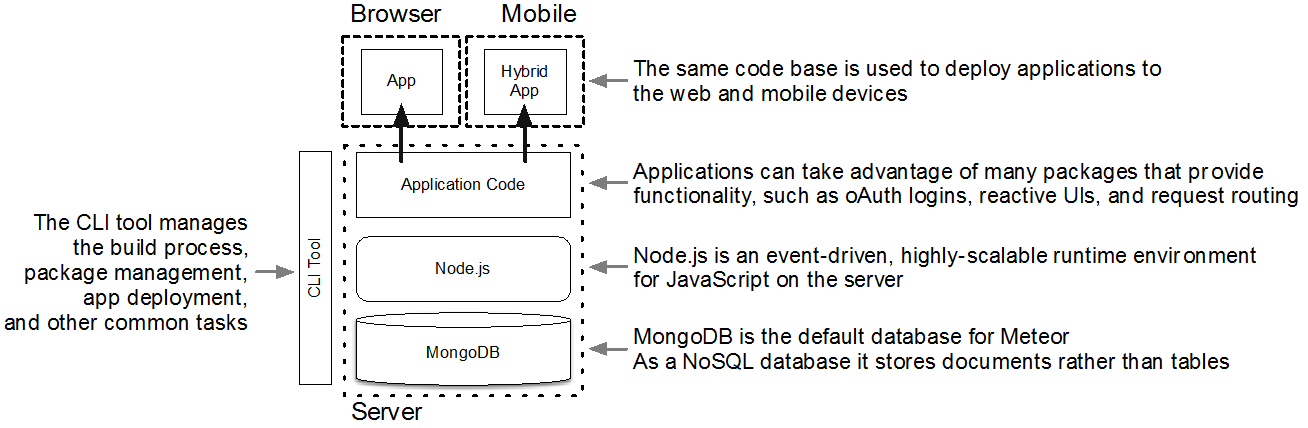
\includegraphics[width=1.0\textwidth]{figuras/meteor_stack.png}
	\caption{El \stackAS \meteorNAME corre aplicaciones potenciadas por \packages inteligentes sobre \nodejsNAME y \mongodbNAME}
	\label{figure:meteor_stack}
\end{figure}

Toda la información es típicamente guardada dentro de \mongodbNAME. Provee una \api \javaScriptNAME que da acceso a todo el contenido almacenado en forma de \documentsDB ó \objectsPL. El mismo lenguaje dentro del \browserINT puede ser usado para acceder a los datos, el cual \meteorNAME toma ventaja para implementar un verdadero desarrollo \fullstackAS.
%All data is typically stored inside a MongoDB, a document-oriented NoSQL database. There are plans for Meteor to support other (SQL-based) database systems, but currently the only suggested DB is Mongo. It provides a JavaScript-API that gives access to all stored content in form of documents or objects. The same language used inside the browser can be used to access data, which Meteor takes advantage to implement true fullstack development.

Todo el \softwarePC y librerías requeridas para crear aplicaciones \webINT desde cero son agrupados en forma de \packages inteligentes, así los desarrolladores pueden empezar de inmediato. Estos \packages incluyen una librería de interfaz de usuario (\blazemeteor), un manejados de cuentas de usuarios (\accountsmeteor), y mantener a todos los \clientsAS \reactively \updated en \realTimeINT (\trackermeteor).
%All required software and libraries required to create web applications from scratch are bundled in the shape of Smart Packages, so developers can get started right away. These packages include a user interface library (Blaze), managing user accounts (accounts), and keeping all clients reactively updated in realtime (Tracker).

La herramienta \clitool de \meteorNAME permite a los desarrolladores rápidamente \setup un \environmentPL completo de desarrollo. No es necesario saber como instalar o configurar algún \softwarePC de \serverAS. \meteorNAME cuida literalmente los aspectos de la infraestructura. Esto es también una herramienta para construir, comparable a \maketool ó \grunttool, y un manejador de \package, tal como \apttool ó \npm. Finalmente la herramienta \clitool agrupa una aplicación para correr en diferentes plataformas de \clientsAS, dentro de un \browserINT \webINT ó como una aplicación \mobileINT nativa.
%The Meteor CLI tool allows developers to quickly set up an entire development environment. There is no need to know how to install or configure any server software, Meteor takes care of the infrastructure aspect entirely. It is also both a build tool, comparable to make or grunt, and a package manager, such as apt or npm. For example it can compile LESS or CoffeeScript on the fly, without first setting up workflow or add authentication via Facebook oAuth with a single command. Finally the CLI tool bundles an application to run on different client platforms, inside a web browser or as native mobile apps.

Todas las partes del \stackAS se integran sin problemas, todos los \packages \coreAS son diseñados y probados para trabajar bien en conjunto. Por otro lado, es perfectamente posible cambiar partes del \stackAS a otros, en caso de ser necesario. En lugar de utilizar \meteorNAME en su totalidad podría decidir utilizarse sólo los componentes de \serverAS y utilizar por ejemplo \angularjsNAME para el \clientSideAS, o utilizar un \javabackend que utilice \meteorNAME en el \frontEndAS para proveer \updates \realTimeINT para todos los \clientsAS.
%All parts of the stack integrate seamlessly, all core packages are designed and tested to work well together. On the other hand, it is entirely possible to switch out parts of the stack for others, should the need arise. Instead of using Meteor in full you could decide to only use the server components and use e.g. Angular.js on the client side, or use a Java-backend that uses Meteor on the front-end to provide realtime updates to all clients. 

\section{\frameworkPC Isomorfo – \fullstackAS \javaScriptNAME}
%Isomorphic Frameworks – Fullstack JavaScript

\meteorNAME corre sobre \nodejsNAME y mueve la lógica de la aplicación hacia el \browserINT, lo que es usualmente referido a \singlePageAppINT. El mismo lenguaje es usado sobre todo el \stackAS, lo que transforma a \meteorNAME en una plataforma Isomorfa. Como resultado el mismo código \javaScriptNAME puede ser usado en el \serverAS, en el \clientAS, e incluso en la \dataBaseDB.
%Meteor runs on top of Node.js and moves the application logic to the browser, which is often referred to as Single Page Applications. The same language is used across the entire stack, which makes Meteor an isomorphic platform. As a result the same JavaScript code can be used on the server, the client, and even in the database. 

Mientras muchos \frameworksPC usan el mismo lenguaje en tanto en \clientAS como en \serverAS, la mayoría del tiempo estos no pueden compartir código porque los \frameworksPC no son íntimamente integrados, por ejemplo el uso de \angularjsNAME en el \frontEndAS y \expressjsNAME en el \backend. \meteorNAME es un \fullstackAS verdadero porque usa una simple y unificada \api expuesta para todas las funcionalidades \coreAS y pueden ser utilizadas en el \serverAS, en el \browserINT, e incluso para acceder a la \dataBaseDB. Para comenzar, no es necesario aprender múltiples \frameworksPC y da como resultado una mejor \reusability del código solo utilizando el mismo lenguaje.
%While many frameworks use the same language on both client and server, most of the times they cannot share code between the two instances because the frameworks are not tightly integrated, for example they use Angular on the frontend and Express.js on the backend. Meteor is truly fullstack because it uses a simple and unified API that exposes all core functionality and can be used on the server, in the browser, and even to access the database. To get started you do not have to learn multiple frameworks and results in much better re-usability of the code than only using the same language.

Para acceder a la \dataBaseDB desde el \browserINT, \meteorNAME incluye una mini \dataBaseDB. Esta simula exactamente la misma \api de una \dataBaseDB. Dentro del \browserINT \minimongo permite a los desarrolladores utilizar los mismos comandos como si estuvieran en una consola de \mongodbNAME.
%To access the database from the browser, Meteor includes mini  databases. They simulate the exact same API of a database. Inside the browser Minimongo allows developers to use the same commands as they would in a MongoDB console.

Típicamente los desarrolladores necesitan saber como escribir código que tome una completa ventaja del \eventloopCPT y que funciones corren \synchronously y cuales \asynchronously (\nameref{cap:section:nodejs}). Mientras mas funcionalidades \asynchronously son utilizadas, tanto mayor serán los \callbacksPL envueltos y las cosas se vuelven bastante sucias.
%Typically, developers need to know how to write code that takes full advantage of the event loop and what functions run synchronously and which asynchronously. The more asynchronous functionality is used, the more callbacks are involved and things can become quite messy.

Afortunadamente, \meteorNAME aprovecha toda la potencia de \eventloopCPT, pero facilita el proceso evitando cierta preocupación sobre escribir código \asynchronousCPT. Utiliza el concepto llamado \fibers \behindthescenes. \fibers proveen una capa de abstracción para el \eventloopCPT que ejecuta funciones \asynchronousCPT(\tasks) en secuencia. Esto elimina la necesidad de \callbacksPL explícitos de manera que se puedan utilizar un estilo \synchronousCPT familiar.
%Fortunately, Meteor leverages the full power of the event loop, but it makes it easy by not having to worry so much about writing asynchronous code. It uses a concept called Fibers behind the scenes. Fibers provide an abstraction layer for the Event Loop that executes asynchronous functions (tasks) in sequence.It removes the need for explicit callbacks so that a familiar synchronous style may be used.

